\paragraph*{ПИД-регулятор угла поворота\\}
\hspace*{\parindent}Введем пропорционально-интегрально-дифференциальный (ПИД) регулятор с передаточной функцией $R(s)$:
\begin{equation}
	R(s)=k_p+k_i\frac{1}{s}+k_ds.
\end{equation}
На рис.~\ref{pid} изображена схема моделирования системы с таким регулятором.

\begin{figure}[h]
	\noindent\centering{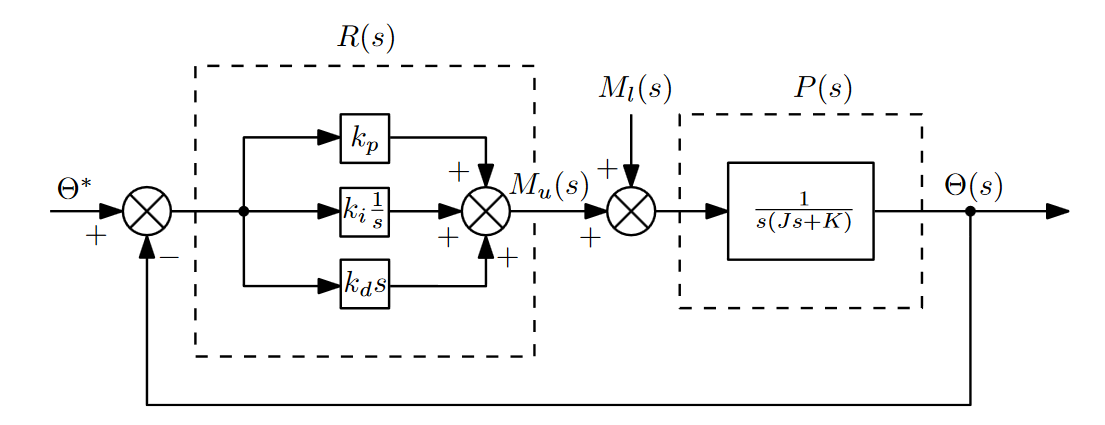
\includegraphics[height = 6cm]{img/mod.png}}
	\caption{Схема моделирования системы с ПИД-регулятором}
	\label{pid}
\end{figure}

\hspace*{\parindent}Выразим из нее выходную переменную:
\begin{equation}
	\Theta(s)=(\Theta^*(s)-\Theta(s))R(s)P(s)-M_l(s))P(s),
\end{equation}
\begin{equation}
	\Theta(s)+\Theta(s)R(s)P(s)=\Theta^*R(s)P(s)-M_l(s)P(s),
\end{equation}
\begin{equation}
	\Theta(s)=\frac{R(s)P(s)}{1+R(s)P(s)}\Theta^*(s)-\frac{P(s)}{1+R(s)P(s)}M_l(s),
\end{equation}
где $\Theta^*(s)$ - желаемый угол поворота.

Рассчитаем передаточную функцию системы при $M_l(s)=0$:
\begin{equation}\label{pidfunc}
	W(s)=\frac{\Theta(s)}{\Theta^*(s)}=\frac{R(s)P(s)}{1+R(s)P(s)}=\frac{\frac{k_ds^2+k_ps+k_i}{J_ms^3+Ks^2}}{1+\frac{k_ds^2+k_ps+k_i}{J_ms^3+Ks^2}}=\frac{k_ds^2+k_ps+k_i}{J_ms^3+(K+k_d)s^2+k_ps+k_i}
\end{equation}

Корни полинома в числителе передаточной функции называются нулями, а корни полинома в знаменателе – полюсами. Знаменатель передаточной функции является характеристическим полиномом дифференциального уравнения движения системы. На основании корней характеристического полинома $J_ms^3+(K+k_d)s^2+k_ps+k_i$ передаточной функции \eqref{pidfunc}, зная значения $J_m$ и $K$,  можно рассчитать такие коэффициенты ПИД-регулятора, чтобы обеспечивались требуемые показатели качества системы. 

\paragraph*{ПИ-регулятор угловой скорости\\}
\hspace*{\parindent}Аналогично, можно вывести регулятор угловой скорости. Сначала, из \eqref{pfunction} получим функцию для угловой скорости:
\begin{equation}
	\Omega(s)=s\Theta(s)=\frac{1}{J_ms+K}(M_u(s)-M_l(s))=P^1(s)(M_u(s)-M_l(s))
\end{equation}

\begin{figure}[h]
	\noindent\centering{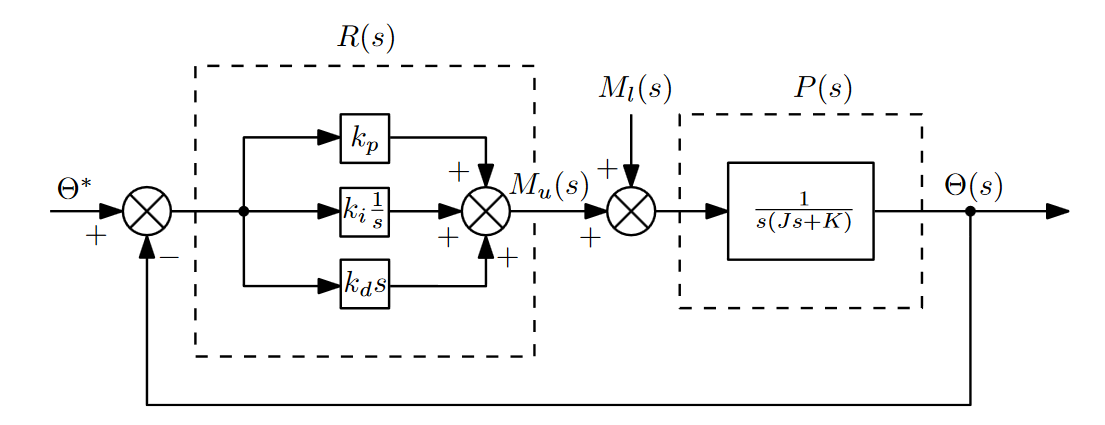
\includegraphics[height = 6cm]{img/mod2.png}}
	\caption{Схема моделирования системы с ПИ-регулятором}
	\label{pi}
\end{figure}

Введем ПИ-регулятор с передаточной функцией:
\begin{equation}
	R^1(s)=k_p^1+k_i^1\frac{1}{s}
\end{equation}
На рис.~\ref{pi} изображена схема моделирования системы с таким регулятором.

Аналогично \eqref{pidfunc}, получим передаточную функцию системы:
\begin{equation}\label{pifunc}
	W^1(s)=\frac{\Omega(s)}{\Omega(s)^*}=\frac{R^1(s)P^1(s)}{1+R^1(s)P^1(s)}=\frac{\frac{k_p^1s+k_i^1}{J_ms^2+Ks}}{1+\frac{k_p^1s+k_i^1}{J_ms^2+Ks}}=\frac{k_p^1s+k_i^1}{J_ms^2+(K+k_p^1)s+k_i^1},
\end{equation}
где $\Omega^*(s)$ - желаемая скорость поворота.

На основании корней характеристического полинома $J_ms^2+(K+k_p^1)s+k_i^1$ передаточной функции \eqref{pifunc} можно рассчитать такие коэффициенты ПИ-регулятора, чтобы обеспечивались требуемые показатели качества системы. Рассмотрим, как это можно сделать. 